% !TEX TS-program = pdflatex
% !TEX encoding = UTF-8 Unicode

% This is a simple template for a LaTeX document using the "article" class.
% See "book", "report", "letter" for other types of document.


\documentclass[10pt]{article} % use larger type; default would be 10pt

\usepackage[utf8]{inputenc} % set input encoding (not needed with XeLaTeX)
\usepackage{float}
%%% Examples of Article customizations
% These packages are optional, depending whether you want the features they provide.
% See the LaTeX Companion or other references for full information.

%%% PAGE DIMENSIONS
\usepackage{geometry} % to change the page dimensions
\geometry{a4paper} % or letterpaper (US) or a5paper or....
% \geometry{margin=2in} % for example, change the margins to 2 inches all round
% \geometry{landscape} % set up the page for landscape
%   read geometry.pdf for detailed page layout information

\usepackage{graphicx} % support the \includegraphics command and options

% \usepackage[parfill]{parskip} % Activate to begin paragraphs with an empty line rather than an indent

%%% PACKAGES
\usepackage{booktabs} % for much better looking tables
\usepackage{array} % for better arrays (eg matrices) in maths
\usepackage{paralist} % very flexible & customisable lists (eg. enumerate/itemize, etc.)
\usepackage{verbatim} % adds environment for commenting out blocks of text & for better verbatim
\usepackage{subfig} % make it possible to include more than one captioned figure/table in a single float
% These packages are all incorporated in the memoir class to one degree or another...
 \usepackage{longtable} % longtable support required by pandoc >1.10
%%% HEADERS & FOOTERS
\usepackage{fancyhdr} % This should be set AFTER setting up the page geometry
\pagestyle{fancy} % options: empty , plain , fancy
\renewcommand{\headrulewidth}{0pt} % customise the layout...
\lhead{}\chead{}\rhead{}
\lfoot{}\cfoot{\thepage}\rfoot{}

%%% SECTION TITLE APPEARANCE
\usepackage{sectsty}
\allsectionsfont{\sffamily\mdseries\upshape} % (See the fntguide.pdf for font help)
% (This matches ConTeXt defaults)

%%% ToC (table of contents) APPEARANCE
\usepackage[nottoc,notlof,notlot]{tocbibind} % Put the bibliography in the ToC
\usepackage[titles,subfigure]{tocloft} % Alter the style of the Table of Contents
\renewcommand{\cftsecfont}{\rmfamily\mdseries\upshape}
\renewcommand{\cftsecpagefont}{\rmfamily\mdseries\upshape} % No bold!
\usepackage[table,xcdraw]{xcolor}
\usepackage{cite}
%%% END Article customizations

%%% The "real" document content comes below...

\title{Functional Annotation of Rare and Low Frequency variants on putative enhancer regions identified by HiCap methods}
\author{Sailendra Pradhananga\\
Science for Life Laboratory/School of Biotechnology\\
Royal KTH institute of Technology (KTH), Swden}
\date{} % Activate to display a given date or no date (if empty),
         % otherwise the current date is printed 

\begin{document}
\maketitle


\section*{Abstract}

Enhancers are non coding DNA elements essential for regulation of genes \cite{shlyueva2014transcriptional}. However they are functional after genome looping which brings distant regions in closer proximity to promoter of genes. Variants in these regions are already implicated in complex diseases. In current study, we have identified common, low frequency and rare variants on HiCap data on two replicates of Bicuspid aortic valve (BAV) heart disease in promoter enhancer interaction genome. The study shows that rare variants are enriched in promoter-mediated putative enhancer. Further annotation of these regions with non coding functional elements with HUVEC cell-line  data set reveals at least  $23\%$ these enhancers are overlapped with at least one of noncoding markers. Gene Ontology term analysis  with promoter enhancer interaction (PEI) genes reveals regulation of endothelial tube morphogenesis as one of the top GO term enriched with Low and rare frequency variants.

\section{Introduction}
Chip-based genome wide association studies  on complex diseased targeted common variants (frequency $>$ 0.05) which had lead to hypothesis of common variant common disease hypothesis \cite{cirulli2010uncovering} However most of common variants identified within the non-coding are unable to explain causality to complex  disease. On the other end of frequency spectrum, rare and Low frequency  variants, are less studied due to large sample requirement and higher cost of sequencing. Recent studies have shown these genetic variants have higher effect on common diseases as well \cite{cirulli2010uncovering, bomba2017impact, saint}. Furthermore, these  non coding  rare and common variants  have shown to disrupt gene regulation mechanism  in promoter-enhancer regions.\cite{chatterjee2016enhancer, rusu2017type} .

One of method to study of studying looping genome is HiCap (variant of Hi-C) \cite{sahlen2015}. The method identifies promoter-anchored interaction between genomic regions that spatially, however are thousand kilo bases apart. Additionally, these interaction provides connectivity information of for example enhancers with potential genes.. In relation  to other competing technologies, HiCap method generates a genome-wide maps of promoter-anchored chromatin interactions with close to single-enhancer resolution.  Enhancers are the cis acting regulatory elements of non coding genome which are essential for regulation of genes transcription. Since enhancer are functionally important region of non coding genome, variations in these regions are of considerable importance in complex diseases  \cite{krijger2016regulation,zhang2015non}

Biscupid aortic valve (BAV) disease  is most common type of aortic anomaly in adults \cite{siu2010bicuspid}. BAV are heritable traits with high influencing males than females, however genetics is poorly understood with no clear one gene influencing disease, thereby speculating effect of different environmental, genetic and epigenetic factor playing the role in disease \cite{siu2010bicuspid,mordi2012bicuspid}. There has been considerable interest to find genetic markers in understanding the prognosis of disease. 

In the current study, we have imputed genetic variants from recently published 1000 Swedish population  \cite{swegen}  in PEI  genomic region from HiCap data of BAV patients. The genetic profile of rare and low frequency variants in PEI  are from two technical replicates from BAV heart disease patient. We observed overlap of these enhancer with genetic variants to different functional elements from Chipseq atlas for primary endothelial HUVEC cell lines.


\section{Materials and methods}

\subsection{Data acquisition}

Whole genome sequencing variant file (vcf) was accessed from SweGen \cite{swegen} database website \cite{Sewfreq}. As reported these dataset includes the highest quality genetic map of Swedish population. From the resulting vcf file, the SNP data set was filtered using a vcftools \cite{danecek2011variant} in order to separate  genetic variant into single nucleotide polymorphism (SNP) and  insertion/deletion (INDEL) type. Additionally,  only the variants tagged as "PASS" from GATK \cite{gatk2} was further processed . Additionally, dubious genome listed in human genome \cite{li2014toward}  was removed from subsequent analysis.

Additionally , for functional annotation of enhancer regions chipseq atlas \cite{Ohta} data  for DNA hypersensitivity experiments (DNAse HS), H3Kme1  and H327Ac , and transcription factor experiments for HUVEC dataset was accessed. The threshold for experiments was set up at 100 and all the peak files were downloaded.  The DHS have lost their condensed chromatin and are exposed for expression. H3Kme1 and H327Ac are the active markers of  putative enhancers and transcription factor are protein complexes that bind to genome for gene expression. These non coding DNA elements  are putatively functionality markers of potential enhancers. 


\subsection{Definition of Rare and low frequency variant in the population}

The variants from the Swedish population was classified into three separate categories i.e Rare, Low frequency and Common based on the allele frequency  in Swedish  population The variant classification were on the frequency such that variant with MAF\textgreater{}0.05 were classified as "Common", Low frequency with 0.05 \textless{} MAF \textless{} 0.01, Rare variants \textless{} 0.01. However in the rare frequency variants were have removed that private variants that were present within one individual either in homozygous or heterozygous condition



\subsection{HiCap interaction dataset}

HiCap experiments on two replicates from BAV patients were performed. The data were preprocessed with each Promoter$-$Enhancer Interaction (PEI)  pair having at greater than three supporting pairs of p-value $< 0.001$  in earlier experiments. The final output of the PEI data consists of information of promoter and corresponding genes, putative  enhancer position in genome and supporting pair information for each interaction in  two replicates. 
Following the interaction dataset, a customized python script \textit{VCFmanipulation.py}  was developed . The script  takes the interaction file  and vcffile as input and subsets PEI regions into the rare, low frequency and common regions. Furthermore, the output from this file is inputted to  python script \textit{genome\_tf.py} further annotates the DNA elements in these regions based on annotation files donwnloaded from Chipseq atlas. 

\subsection {GO term enrichment status of P\_E interaction mediated genes}

GO term of biological processes (BP) that were curated from the GO database were down from QuickGo \cite{quickgo} . Additionally while downloading  the  BP date, we considered only the terms that were fulfilled the criteria of manual experiment evidence given in the QuickGO database. We used this criteria in order to limit or gene ontologies analysis to relatively functional genes which have the experimental validation. A customized python \textit{Gene\_ontology.py} was made in for the following analysis as well.

\section{Results}

\subsection{Rare variants are enriched in putative Promoter - Enhancer Interaction}
There was 35million variants that were tagged as "Pass" all 1000 Swedish genome population. From that, we have identified around 30.2 million SNPs and 4.4 million indels in in the population that are tagged as "Pass" from GATK filter.

The preprocessed promoter-enhancer list contained 33,323 unique enhancers regions in Bicuspid aortic valve. This data contains of promoter regions and corresponding enhancer regions of 2 replicates from BAV cell. We found on average of 20.38 and 13.93 interaction enhancers change in replicate1 and replicate2 respectively.We observed that enhancer had different length distribution as shown in table~\ref{table1} and fig~\ref{duplcated}. This length distribution depicts that most of our putative enhancers are within the range of 50-1Mb base pairs which is in par with the Hi-C methods

  
\begin{longtable}[]{@{}lcr@{}}
\toprule
 Enhancer\_length & Counts
type\tabularnewline
\midrule
\endhead
$< 50$kb   & 82591\tabularnewline
$50-500$kb   & 20700\tabularnewline
$500$kb $-1$Mb &  3334\tabularnewline
 $> 1$MB & 1030\tabularnewline
\bottomrule
\caption{\small Number of enhancer of different length}
\label{table1}
\end{longtable}

\begin{figure}[H]
\begin{center}
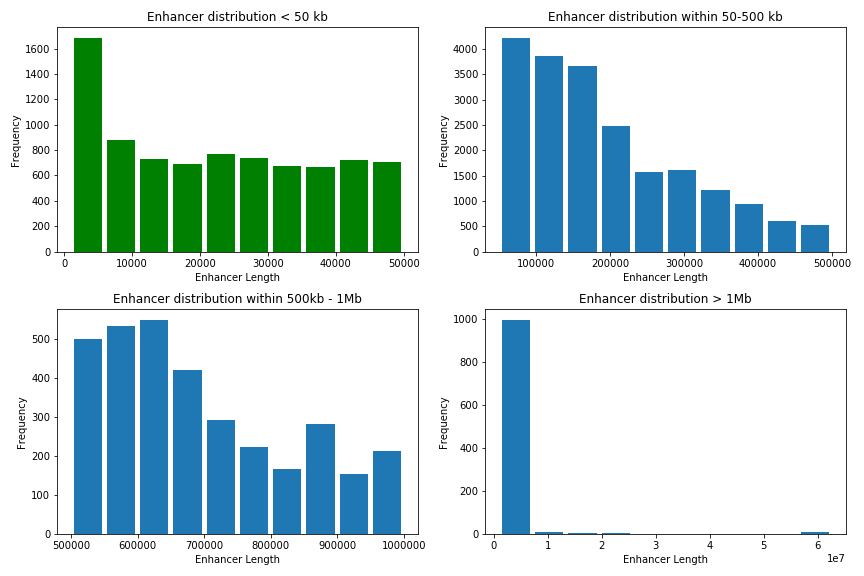
\includegraphics[width=0.9\textwidth]{length_distribution}
\caption{\small Distribution of Enhancer length on PEI dataset. Most of enhancer was between 50 Kb$-$ 1Mb in length}
\label{duplcated}
\end{center}
\end{figure}



We identified  22,055, 14403 and 22,144 putative enhancer regions in our interaction dataset with common, low-frequency and rare variants respectively . Furthermore, we identified in total 56,891 common , 24,049 low-frequency and  47,281 rare variants enriched in these enhancer regions as shown in table~\ref{table2} . Interestingly, our enhancer regions have been enriched with rare variants from Swedish population as compared to other variant class fig~\ref{fig2}.

\begin{longtable}[]{@{}lcr@{}}
\toprule
Variant class & Enhancer with variants & Total variants
type\tabularnewline
\midrule
\endhead
Common & 22055 & 56891\tabularnewline
Low Frequency & 14403 & 24049\tabularnewline
Rare & 22144 & 47281\tabularnewline
\bottomrule
\caption{\small Number of different class of variants in PEI enhancers}
\label{table2}
\end{longtable}

\begin{figure}[H]
\centering
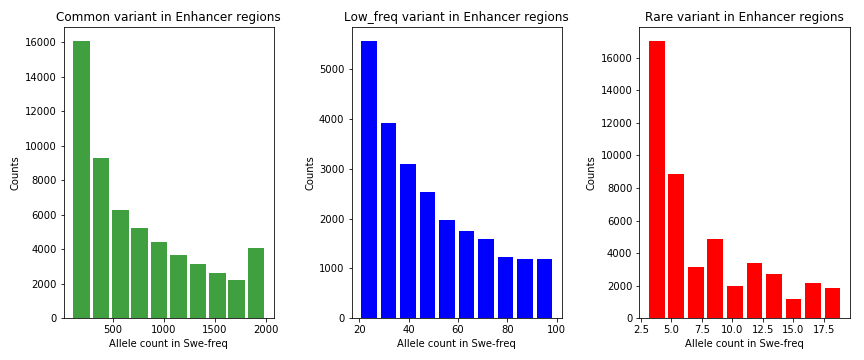
\includegraphics[width=\textwidth]{Distibution_allelecount.png}
\caption{\small Distribution of different variant class in PEI. The number of allele count in Swefreq Database in x$-$axis and count in y$-$axis. Rare variants are enriched with the allele count $<$ 5.}
\label{fig2}
\end{figure}



\subsection{Status of non coding functional DNA elements of variants embedded enhancer regions}

Upon overlapping with the chipseq atlas experimental data with different DNA elements, we all the DNA elements are present in our enhancer list in all classes as shown in table~\ref{table3}. 

\begin{table}[H]
\centering
\begin{tabular}{@{}lllllllll@{}}
\toprule
\rowcolor[HTML]{BBDAFF} 
\multicolumn{1}{c}{\cellcolor[HTML]{BBDAFF}{\color[HTML]{333333} class}} & {\color[HTML]{333333} at\_least\_one} & {\color[HTML]{333333} DNS} & {\color[HTML]{333333} HM} & {\color[HTML]{333333} TFs} & {\color[HTML]{333333} DNS+HM} & {\color[HTML]{333333} DNS+TFs} & {\color[HTML]{333333} HM+TFs} & {\color[HTML]{333333} ALL} \\ \midrule
\cellcolor[HTML]{FFFFFF}Common & 5087 & 3350 & 3029 & 3416 & 2042 & 2487 & 1744 & 1565 \\
\cellcolor[HTML]{FFFFFF}Low Frequency & 3407 & 2276 & 2038 & 2356 & 1393 & 1736 & 1229 & 1095 \\
\cellcolor[HTML]{FFFFFF}Rare & 5178 & 3440 & 3097 & 3524 & 2114 & 2587 & 1820 & 1638 \\ \bottomrule
\end{tabular}
\caption{\small Different DNA elements in enhancer of variant classes Common, Low frequency and Rare}
\label{table3}
\end{table}

Additionally, when we compared types of DNA elements we observed hat we have at least one of functional markers in about (5087/22055) 23\% of putative enhancer in all classes of variants as shown in fig~\ref{fig3}. However, it has to be considered that we took into consideration one of cell line and these are the markers specific to cell type. Most interesting , we still find at least 1000 putatively, functional enhancers in all variant classes. It would be interesting to observe these functional enhancer regions and dig into Rare and Low frequency variants in these region.Furthermore, these are result only from overlapping with one dataset. This data has to be randomized and overlapped so as to find the putative p-values to our non coding functional elements.


\begin{figure}[H]
\centering
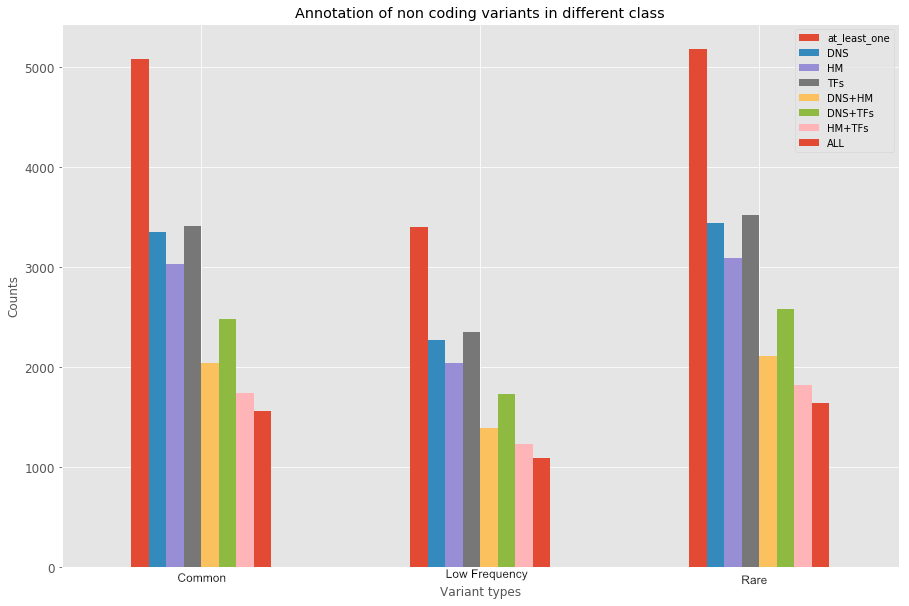
\includegraphics[width=0.85\textwidth]{Enhancer_elements.png}
\caption{\small Distribution of different DNA elements in enhancer with variant classes}
\label{fig3}
\end{figure}




\subsection{GO term enrichment status of PEI mediated genes on variant with all functional markers }

We sub selected the enhancers with all the functional marks as we had observed earlier. Upon Gene Ontology analysis of PEI mediated genes on PEI of variant class rare and low frequency on such enhancers resulted some interesting observations. We found 2 enriched GO Terms at PEI more than two. The top GO enriched terms were 1) \textit {GO:1902894 regulation of pri-miRNA
transcription from RNA polymerase II promoter} and 2) \textit {GO:1901509 regulation of endothelial tube morphogenesis}. 

\section{Discussion}

In the current report we have presented the status of genetic variants identified from Swedish population in the putative enhancer genomic regions mediated by promoter-enhancer mediated interaction (PEI). These PEIs were called using HiCap experiments in replicates of BAV heart disease patient.  Our analysis depicts that rare variants are enriched within our enhancer regions which was as expected since these rare variants also contains the variants which might be presented in one individuals as we haven't corrected for homogenous individuals. However we still find variants which are presented at least greater than five allele counts . 

Based on the definition rare, low frequency and common variants, we annotated our enhancer with active enhancers marks. We used publicly available HUVEC dataset for chipseq atlas on DNAse Hypersensitivity. These regions provided the accessibility of genome for  further processing . In the same enhancers regions we annotated with active enhancers histone marks (H327ac and H3Kme1) and transcription factor binding sites. The formation of complex between TFs, enhancers and promoter have been already reported as fundamental mechanism for regulation of trancription \cite{mora2015loop}.  At the current state of analysis, we find more than  1000 enhancer regions which have been all of these functional marks. This is still a lower number and overlapped within one type of cell-line. Based on the this result, we can regards these enhancers are functional . Furthermore, from this primary analysis, we have to calculate enrichment status based on random distance mediated enhancer.

GO-Term analysis have represented regulation of endothelial tube morphogenesis as one of GO with high enhancer activity in rare and low frequency class of variants. Endothelial progenitor cells have been associated as biomarker of cardiovascular disease \cite{grisar2011endothelial}.  There has been elucidation of endothelial cells in relation to inflammation in vascular disorders. Thus, the genes associated i.e \textit{FOXP1 }and  \textit{FGF1} and their corresponding enhancer could have functional implication in understanding disease prognosis. However these genes and GO term analysis needs further processing on experimental validation.


\section{Conclusion}

We have used currently available large scale genetic frequency data in homogenous Swedish population to identify the promoter mediated enhancer enriched with rare variants. Upon further annotation of these enhancer with functional markers lead to identification of interesting GO-terms. Although HiCap based enhancer analysis is currently fully mature, we believe that preliminary results points that rare variants could potentially driving the complex phenotypes such as BAV heart disease.



\newpage

\bibliographystyle{IEEEtran}
%\bibliographystyle{unsrt}
\bibliography{report_17th_Oct}



















\end{document}
